\documentclass[tikz,border=6pt]{standalone}
\usepackage[T1]{fontenc}
\usepackage{lmodern}
\usepackage{amsmath,amssymb}
\usetikzlibrary{positioning,arrows.meta,fit,calc}
% Design of koblitz-n83-indexlift-20261019 (frozen protocol.json). Not a result.
\begin{document}
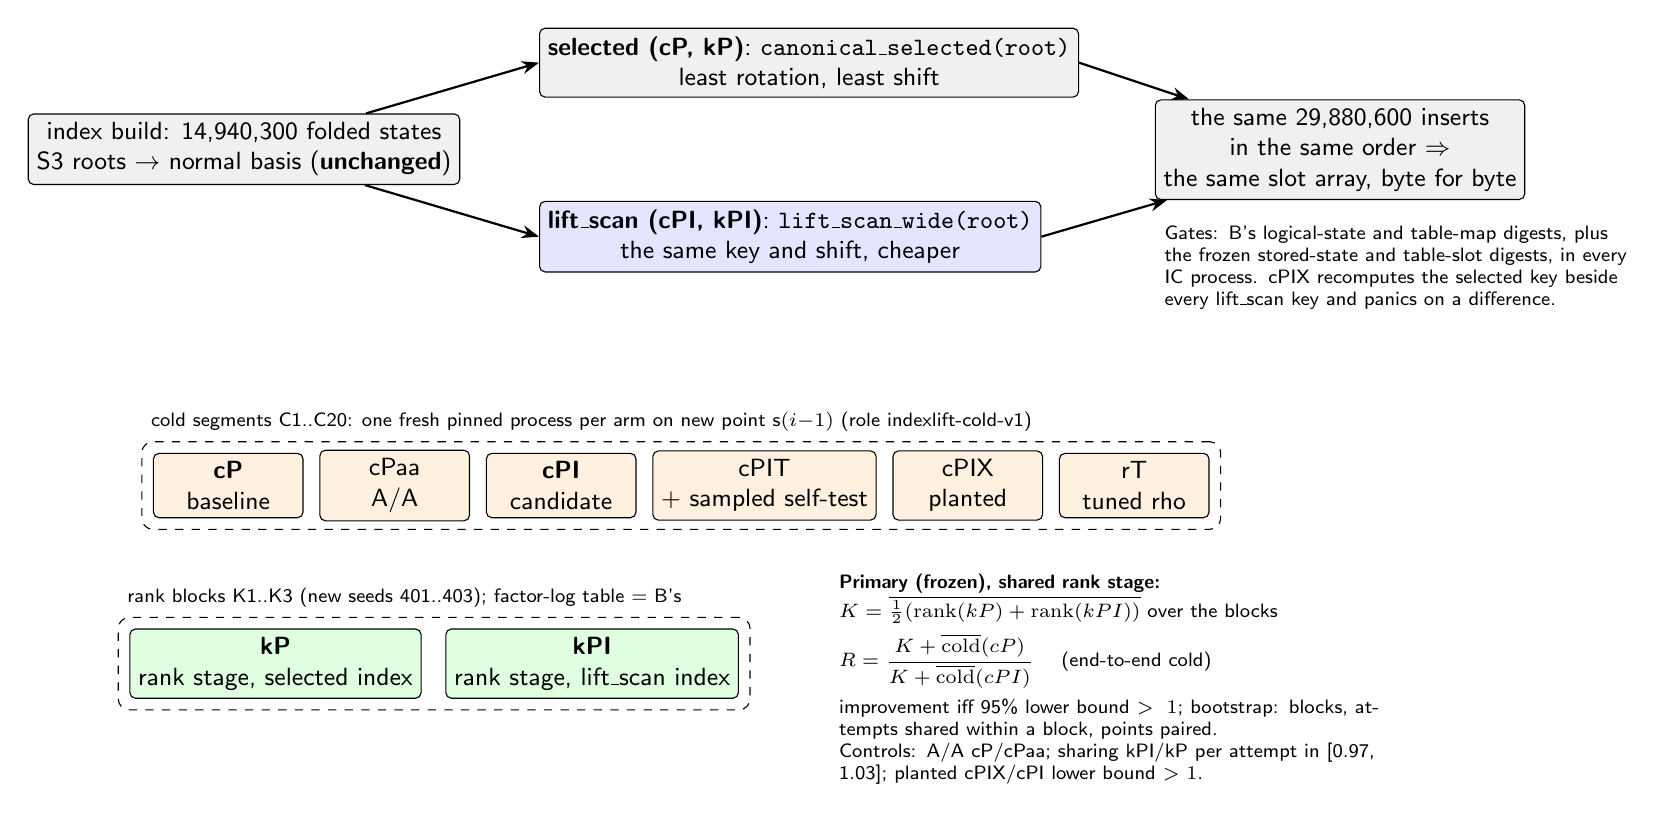
\begin{tikzpicture}[
  font=\sffamily\small,
  box/.style={draw, rounded corners=2pt, align=center, minimum height=8mm, inner sep=3pt},
  base/.style={box, fill=gray!12},
  add/.style={box, fill=blue!10},
  arm/.style={box, fill=orange!12, minimum width=19mm},
  rank/.style={box, fill=green!12, minimum width=30mm},
  arr/.style={-{Stealth[length=2.2mm]}, thick},
  note/.style={align=left, font=\sffamily\scriptsize}
]
% Index build of one process
\node[base] (st) {index build: 14,940,300 folded states\\S3 roots $\to$ normal basis (\textbf{unchanged})};
\node[base, above right=2mm and 10mm of st] (sel) {\textbf{selected (cP, kP)}: \texttt{canonical\_selected(root)}\\least rotation, least shift};
\node[add, below right=2mm and 10mm of st] (lift) {\textbf{lift\_scan (cPI, kPI)}: \texttt{lift\_scan\_wide(root)}\\the same key and shift, cheaper};
\draw[arr] (st) -- (sel.west); \draw[arr] (st) -- (lift.west);
\node[base, anchor=west] (tab) at ($(sel.east)!0.5!(lift.east) + (12mm,0)$) {the same 29,880,600 inserts\\in the same order $\Rightarrow$\\the same slot array, byte for byte};
\draw[arr] (sel.east) -- (tab); \draw[arr] (lift.east) -- (tab);
\node[note, anchor=north west, text width=60mm] at ($(tab.south west)+(0mm,-2mm)$) {Gates: B's logical-state and table-map digests, plus the frozen stored-state and table-slot digests, in every IC process. cPIX recomputes the selected key beside every lift\_scan key and panics on a difference.};

% Cold arms
\node[arm, below=34mm of st, xshift=-2mm] (cP) {\textbf{cP}\\baseline};
\node[arm, right=2mm of cP] (cPaa) {cPaa\\A/A};
\node[arm, right=2mm of cPaa] (cPI) {\textbf{cPI}\\candidate};
\node[arm, right=2mm of cPI] (cPIT) {cPIT\\+ sampled self-test};
\node[arm, right=2mm of cPIT] (cPIX) {cPIX\\planted};
\node[arm, right=2mm of cPIX] (rT) {rT\\tuned rho};
\node[draw, dashed, rounded corners, fit=(cP) (rT), inner sep=4pt, label={[note, anchor=south west]north west:{cold segments C1..C20: one fresh pinned process per arm on new point s$(i{-}1)$ (role indexlift-cold-v1)}}] (cold) {};

% Rank arms
\node[rank, below=14mm of cP, xshift=6mm] (kP) {\textbf{kP}\\rank stage, selected index};
\node[rank, right=3mm of kP] (kPI) {\textbf{kPI}\\rank stage, lift\_scan index};
\node[draw, dashed, rounded corners, fit=(kP) (kPI), inner sep=4pt, label={[note, anchor=south west]north west:{rank blocks K1..K3 (new seeds 401..403); factor-log table = B's}}] (rk) {};

\node[note, anchor=west, text width=74mm] (eq) at ($(rk.east)+(10mm,-2mm)$) {\textbf{Primary (frozen), shared rank stage:}\\
$K=\overline{\tfrac12(\mathrm{rank}(kP)+\mathrm{rank}(kPI))}$ over the blocks\\[1mm]
$R = \dfrac{K + \overline{\mathrm{cold}}(cP)}{K + \overline{\mathrm{cold}}(cPI)}$ \quad (end-to-end cold)\\[1mm]
improvement iff 95\% lower bound $>1$; bootstrap: blocks, attempts shared within a block, points paired.\\
Controls: A/A cP/cPaa; sharing kPI/kP per attempt in [0.97, 1.03]; planted cPIX/cPI lower bound $>1$.};
\end{tikzpicture}
\end{document}
